%%%%%%%%%%%%%%%%%%%%%%%%%%ch3-3
\begin{frame}[shrink]
  \frametitle{ch3.信号检测与估计理论的基础知识}
  \framesubtitle{ch3-3. 贝叶斯准则---例题(续)及性能分析}
  \tableofcontents[hideallsubsections]
\end{frame}

\section{贝叶斯准则例题4}

\begin{frame}{贝叶斯准则例题4}
考虑以下信号检测问题:
\begin{align*}
H_0: x_k&=1+n_{k},   & k=1,2,\dots,N\\
H_1: x_k&=-1+n_{k}, & k=1,2,\dots,N
\end{align*}
其中$n_{k}$是均值为零,方差为$\sigma_n^2=1/2$的高斯随机变量,  且不同采样时刻的加性噪声之间是相互统计独立的。\\
若两种假设先验等概的,且代价因子为$c_{00}=1, c_{10}=4, c_{11}=2, c_{01}=3$。\\
请给出上述问题的贝叶斯检测准则和平均代价$C$。
\end{frame}

\begin{frame}[shrink]{贝叶斯准则例题4: 判决概率分布分析}
\begin{columns}
	\column{0.5\textwidth}
	\begin{align*}
	&H_0: x_k=1+n_k,\quad H_1: x_k=-1+n_k\\
	&k=1,2,\dots,N,\quad \bm{x}=(x_1,x_2,\dots,x_N)^{T}\\
	&P(H_i|H_j)=\int_{R_i}p(\bm{x}|H_j)d\bm{x}
	\end{align*}
	\column{0.5\textwidth}
	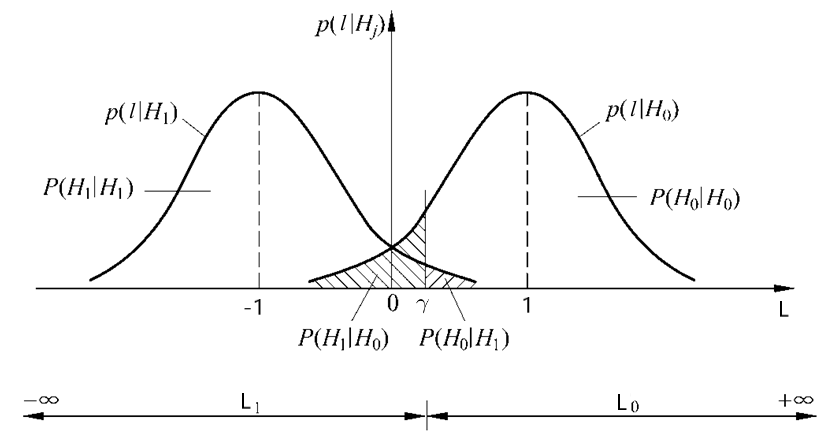
\includegraphics[scale=0.23]{detectionL-1}
\end{columns}
\begin{align*}
&P(H_0|H_0)=\int_{L_0}p(\bm{x}|H_0)d\bm{x},\qquad P(H_1|H_0)=\int_{L_1}p(\bm{x}|H_0)d\bm{x}\\
&P(H_0|H_1)=\int_{L_0}p(\bm{x}|H_1)d\bm{x},\qquad P(H_1|H_1)=\int_{L_1}p(\bm{x}|H_1)d\bm{x}\\
&\bm{L}=L_0\cup L_1,\quad L_0\cap L_1=\emptyset, \quad \int_{\bm{L}}p(\bm{x}|H_j)d\bm{x}=1\\
&P(H_0|H_0)+P(H_1|H_0)=\int_{L_0}p(\bm{x}|H_0)d\bm{x}+\int_{L_1}p(\bm{x}|H_0)d\bm{x}=\int_{\bm{L}}p(\bm{x}|H_0)d\bm{x}=1\\
&P(H_0|H_1)+P(H_1|H_1)=\int_{L_0}p(\bm{x}|H_1)d\bm{x}+\int_{L_1}p(\bm{x}|H_1)d\bm{x}=\int_{\bm{L}}p(\bm{x}|H_1)d\bm{x}=1
\end{align*}
\end{frame}

\begin{frame}[shrink]{贝叶斯准则例题4: 解}
解: $N$次独立采样, 样本为$x_k(k=1,2,\cdots,N)$:
\begin{align*}
H_0: x_k&=1+n_k && k=1,2,\cdots,N\\
H_1: x_k&=-1+n_k && k=1,2,\cdots,N
\end{align*}
\textbf{步骤1: 计算两个似然函数, 构建似然比}\\
由于$n$是高斯分布随机变量, 因此在$H_0$假设下, 第$k$次采样值$x_k$服从高斯分布,且均值为1, 方差为$\sigma_n^2$; 在$H_1$假设下, 第$k$次采样值$x_k$服从均值为$-1$, 方差为$\sigma_n^2$的高斯分布。
\begin{align*}
p(x_k|H_0)&=\left(\frac{1}{2\pi\sigma_n^2}\right)^{1/2}\exp\left(-\frac{(x_k-1)^2}{2\sigma_n^2}\right)\implies p(\bm{x}|H_0)=\prod_{k=1}^{N}\left(\frac{1}{2\pi\sigma_n^2}\right)^{1/2}\exp\left(-\frac{(x_k-1)^2}{2\sigma_n^2}\right)\\
p(x_k|H_1)&=\left(\frac{1}{2\pi\sigma_n^2}\right)^{1/2}\exp\left(-\frac{(x_k+1)^2}{2\sigma_n^2}\right)\implies p(\bm{x}|H_1)=\prod_{k=1}^{N}\left(\frac{1}{2\pi\sigma_n^2}\right)^{1/2}\exp\left(-\frac{(x_k+1)^2}{2\sigma_n^2}\right)\\
\lambda(\bm{x})&=\frac{p(\bm{x}|H_1)}{p(\bm{x}|H_0)}=\exp\left(\frac{\sum\limits_{k=1}^{N}\left((x_k-1)^2-(x_k+1)^2\right)}{2\sigma_n^2}\right)
\end{align*} 
\end{frame}

\begin{frame}[shrink]{贝叶斯准则例题4: 解续(1)}
\textbf{步骤2: 根据两个假设的先验概率和代价因子, 计算判决门限}
\[\eta\mathop{=}\limits^{def}\frac{P(H_0)(c_{10}-c_{00})}{P(H_1)(c_{01}-c_{11})}=\frac{4-1}{3-2}=3 \]
\textbf{步骤3: 形成贝叶斯检测基本表达式}
\begin{align*}
\lambda(\bm{x})=\frac{p(\bm{x}|H_1)}{p(\bm{x}|H_0)}&\mathop{\gtrless}\limits_{H_0}^{H_1}\eta\\
\exp\left(\frac{\sum\limits_{k=1}^{N}\left((x_k-1)^2-(x_k+1)^2\right)}{2\sigma_n^2}\right)&\mathop{\gtrless}\limits_{H_0}^{H_1}\eta
\end{align*} 
\textbf{步骤4: 化简, 形成贝叶斯检测判决表达式}
\begin{align*}
-4\sum\limits_{k=1}^{N}x_k\mathop{\gtrless}\limits_{H_0}^{H_1}2\sigma_n^2\ln\eta\implies \sum\limits_{k=1}^{N}x_k\mathop{\gtrless}\limits_{H_1}^{H_0}-\frac{\sigma_n^2\ln\eta}{2}\\
l(\bm{x})\mathop{=}^{def}\frac{1}{N}\sum\limits_{k=1}^{N}x_k\mathop{\gtrless}\limits_{H_1}^{H_0}-\frac{\sigma_n^2\ln\eta}{2N}=-\frac{\ln3}{4N}\mathop{=}^{def}\gamma\\
\end{align*} 
\end{frame}

\begin{frame}[shrink]{贝叶斯准则例题4: 解续(2)}
经过上述化简, 信号检测的判决式由似然比检验的形式, 简化为检验统计量$l(x)$与检测门限$\gamma$相比较的形式, 形成贝叶斯检测判决表达式:
\[
l(\bm{x})\mathop{=}^{def}\frac{1}{N}\sum\limits_{k=1}^{N}x_k\mathop{\gtrless}\limits_{H_1}^{H_0}-\frac{\sigma_n^2\ln\eta}{2N}=-\frac{\ln3}{4N}\mathop{=}^{def}\gamma
\]
检验统计量$l(x)\mathop{=}\limits^{def}\frac{1}{N}\sum\limits_{k=1}^Nx_k$是观测信号$x_k(k=1,2,\dots,N)$的求和取平均值的结果, 即它是$x_k(k=1,2,\dots,N)$的函数,是一个随机变量。\\
因为高斯随机变量的线性组合还是高斯随机变量,  所以两种假设下的观测量$(l|H_0),(l|H_1)$也是服从高斯分布的随机变量。
\end{frame}

\begin{frame}[shrink]{贝叶斯准则例题4: 性能分析---观测量$(l|H_0)$}
\begin{columns}
	\column{0.21\textwidth}
	$H_0:x_k=1+n_k$\\
	$H_1:x_k=-1+n_k$
	\column{0.79\textwidth}
	\[
	l(\bm{x})\mathop{=}^{def}\frac{1}{N}\sum\limits_{k=1}^{N}x_k\mathop{\gtrless}\limits_{H_1}^{H_0}-\frac{\sigma_n^2\ln\eta}{2N}=-\frac{\ln3}{4N}\mathop{=}^{def}\gamma \quad \textbf{统计量: }l(\bm{x})\mathop{=}\limits^{def}\frac{1}{N}\sum\limits_{k=1}^{N}x_k
	\]
\end{columns}
\textbf{假设$H_0$条件下, 统计量$l(x)$为高斯分布, 均值和方差分别为}
\begin{align*}
E[l|H_0]&=E\left[\frac{1}{N}\sum\limits_{k=1}^{N}(x_k|H_0)\right]=E\left[\frac{1}{N}\sum\limits_{k=1}^{N}(1+n_k)\right]=\frac{1}{N}\sum\limits_{k=1}^{N}E[1+n_k]=1\\
Var[l|H_0]&=E\left[(l|H_0-E(l|H_0))^2\right]=E\left[\left(\frac{1}{N}\sum\limits_{k=1}^{N}(1+n_k)-1\right)^2\right]\\
&=\frac{1}{N^2}\sum\limits_{k=1}^{N}E[n_k^2]=\frac{1}{N^2}\sum\limits_{k=1}^{N}\sigma_n^2=\frac{\sigma_n^2}{N}
\end{align*}
\textbf{因此, }$(l|H_0)\sim\mathcal{N}(1,\frac{\sigma_n^2}{N})$
\begin{align*}
p(l|H_0)=\left(\frac{1}{2\pi Var[l|H_0]}\right)^{1/2}\exp\left(-\frac{(l-E[l|H_0])^2}{2 Var[l|H_0]}\right)=\left(\frac{N}{2\pi\sigma_n^2}\right)^{1/2}\exp\left(-\frac{N(l-1)^2}{2\sigma_n^2}\right)
\end{align*}
\end{frame}

\begin{frame}[shrink]{贝叶斯准则例题4: 性能分析---观测量$(l|H_0)$}
\begin{columns}
	\column{0.21\textwidth}
	$H_0:x_k=1+n_k$\\
	$H_1:x_k=-1+n_k$
	\column{0.79\textwidth}
	\[
	l(\bm{x})\mathop{=}^{def}\frac{1}{N}\sum\limits_{k=1}^{N}x_k\mathop{\gtrless}\limits_{H_1}^{H_0}-\frac{\sigma_n^2\ln\eta}{2N}=-\frac{\ln3}{4N}\mathop{=}^{def}\gamma \quad \textbf{统计量: }l(\bm{x})\mathop{=}\limits^{def}\frac{1}{N}\sum\limits_{k=1}^{N}x_k
	\]
\end{columns}
\begin{align*}
p(l|H_0)=\left(\frac{N}{2\pi\sigma_n^2}\right)^{1/2}\exp\left(-\frac{N(l-1)^2}{2\sigma_n^2}\right)
\end{align*}
\begin{align*}
P(H_1|H_0)&=1-\int_{\gamma}^{\infty}p(l|H_0)dl\implies Q(u)=\int_{x}^{\infty}\left(\frac{1}{2\pi}\right)^{1/2}\exp\left(-\frac{u^2}{2}\right)du\\
&=1-\int_{\gamma}^{\infty}\left(\frac{N}{2\pi\sigma_n^2}\right)^{1/2}\exp\left(-\frac{N(l-1)^2}{2\sigma_n^2}\right)dl\qquad \text{by } l=\frac{\sigma_nu}{\sqrt{N}}+1\\
&=1-\int_{\frac{\sqrt{N}(\gamma-1)}{\sigma_n}}^{\infty}\left(\frac{1}{2\pi}\right)^{1/2}\exp\left(-\frac{u^2}{2}\right)du\\
&=1-Q\left(\frac{\sqrt{N}(\gamma-1)}{\sigma_n}\right)=1-Q\left(\frac{\sqrt{N}\left(-\frac{\sigma_n^2\ln\eta}{2N}-1\right)}{\sigma_n}\right)
\end{align*}
\end{frame}

\begin{frame}[shrink]{贝叶斯准则例题4: 性能分析---观测量$(l|H_0)$}
\begin{columns}
	\column{0.21\textwidth}
	$H_0:x_k=1+n_k$\\
	$H_1:x_k=-1+n_k$
	\column{0.79\textwidth}
	\[
	l(\bm{x})\mathop{=}^{def}\frac{1}{N}\sum\limits_{k=1}^{N}x_k\mathop{\gtrless}\limits_{H_1}^{H_0}-\frac{\sigma_n^2\ln\eta}{2N}=-\frac{\ln3}{4N}\mathop{=}^{def}\gamma \quad \textbf{统计量: }l(\bm{x})\mathop{=}\limits^{def}\frac{1}{N}\sum\limits_{k=1}^{N}x_k
	\]
\end{columns}
\begin{align*}
P(H_1|H_0)&=1-Q\left(\frac{\sqrt{N}\left(-\frac{\sigma_n^2\ln\eta}{2N}-1\right)}{\sigma_n}\right)\\
&=1-Q\left(-\frac{\sigma_n\ln\eta}{2\sqrt{N}}-\frac{\sqrt{N}}{\sigma_n}\right)&& \text{by }d^2=\frac{4N}{\sigma_n^2}\\
&=1-Q\left(-\frac{\ln\eta}{d}-\frac{d}{2}\right)\\
P(H_0|H_0)&=1-P(H_1|H_0)
\end{align*}
\end{frame}

\begin{frame}[shrink]{贝叶斯准则例题4: 性能分析---观测量$(l|H_1)$}
\begin{columns}
	\column{0.21\textwidth}
	$H_0:x_k=1+n_k$\\
	$H_1:x_k=-1+n_k$
	\column{0.79\textwidth}
	\[
	l(\bm{x})\mathop{=}^{def}\frac{1}{N}\sum\limits_{k=1}^{N}x_k\mathop{\gtrless}\limits_{H_1}^{H_0}-\frac{\sigma_n^2\ln\eta}{2N}=-\frac{\ln3}{4N}\mathop{=}^{def}\gamma \quad \textbf{统计量: }l(\bm{x})\mathop{=}\limits^{def}\frac{1}{N}\sum\limits_{k=1}^{N}x_k
	\]
\end{columns}
\textbf{假设$H_1$条件下, 统计量$l(x)$为高斯分布, 均值和方差分别为}
\begin{align*}
E[l|H_1]&=E\left[\frac{1}{N}\sum\limits_{k=1}^{N}(x_k|H_1)\right]=E\left[\frac{1}{N}\sum\limits_{k=1}^{N}(-1+n_k)\right]=-1+\frac{1}{N}\sum\limits_{k=1}^{N}E[n_k]=-1\\
Var[l|H_1]&=E\left[(l|H_1-E(l|H_1))^2\right]=E\left[\left(\frac{1}{N}\sum\limits_{k=1}^{N}(-1+n_k)+1\right)^2\right]\\
&=\frac{1}{N^2}\sum\limits_{k=1}^{N}E[n_k^2]=\frac{1}{N^2}\sum\limits_{k=1}^{N}\sigma_n^2=\frac{\sigma_n^2}{N}
\end{align*}
\textbf{因此, }$(l|H_1)\sim\mathcal{N}(-1,\frac{\sigma_n^2}{N})$
\begin{align*}
p(l|H_1)=\left(\frac{1}{2\pi Var[l|H_1]}\right)^{1/2}\exp\left(-\frac{(l-E[l|H_1])^2}{2 Var[l|H_1]}\right)=\left(\frac{N}{2\pi\sigma_n^2}\right)^{1/2}\exp\left(-\frac{N(l+1)^2}{2\sigma_n^2}\right)
\end{align*}
\end{frame}

\begin{frame}[shrink]{贝叶斯准则例题4: 性能分析---观测量$(l|H_1)$}
\begin{columns}
	\column{0.21\textwidth}
	$H_0:x_k=1+n_k$\\
	$H_1:x_k=-1+n_k$
	\column{0.79\textwidth}
	\[
	l(\bm{x})\mathop{=}^{def}\frac{1}{N}\sum\limits_{k=1}^{N}x_k\mathop{\gtrless}\limits_{H_1}^{H_0}-\frac{\sigma_n^2\ln\eta}{2N}=-\frac{\ln3}{4N}\mathop{=}^{def}\gamma \quad \textbf{统计量: }l(\bm{x})\mathop{=}\limits^{def}\frac{1}{N}\sum\limits_{k=1}^{N}x_k
	\]
\end{columns}
\begin{align*}
p(l|H_1)=\left(\frac{N}{2\pi\sigma_n^2}\right)^{1/2}\exp\left(-\frac{N(l+1)^2}{2\sigma_n^2}\right)
\end{align*}
\begin{align*}
P(H_0|H_1)&=\int_{\gamma}^{\infty}p(l|H_1)dl\implies Q(u)=\int_{x}^{\infty}\left(\frac{1}{2\pi}\right)^{1/2}\exp\left(-\frac{u^2}{2}\right)du\\
&=\int_{\gamma}^{\infty}\left(\frac{N}{2\pi\sigma_n^2}\right)^{1/2}\exp\left(-\frac{N(l+1)^2}{2\sigma_n^2}\right)dl\qquad \text{by } l=\frac{\sigma_nu}{\sqrt{N}}-1\\
&=\int_{\frac{\sqrt{N}(\gamma+1)}{\sigma_n}}^{\infty}\left(\frac{1}{2\pi}\right)^{1/2}\exp\left(-\frac{u^2}{2}\right)du\\
&=Q\left(\frac{\sqrt{N}(\gamma+1)}{\sigma_n}\right)=Q\left(\frac{\sqrt{N}\left(-\frac{\sigma_n^2\ln\eta}{2N}+1\right)}{\sigma_n}\right)
\end{align*}
\end{frame}

\begin{frame}[shrink]{贝叶斯准则例题4: 性能分析---观测量$(l|H_1)$}
\begin{columns}
	\column{0.21\textwidth}
	$H_0:x_k=1+n_k$\\
	$H_1:x_k=-1+n_k$
	\column{0.79\textwidth}
	\[
	l(\bm{x})\mathop{=}^{def}\frac{1}{N}\sum\limits_{k=1}^{N}x_k\mathop{\gtrless}\limits_{H_1}^{H_0}-\frac{\sigma_n^2\ln\eta}{2N}=-\frac{\ln3}{4N}\mathop{=}^{def}\gamma \quad \textbf{统计量: }l(\bm{x})\mathop{=}\limits^{def}\frac{1}{N}\sum\limits_{k=1}^{N}x_k
	\]
\end{columns}
\begin{align*}
P(H_0|H_1)&=Q\left(\frac{\sqrt{N}\left(-\frac{\sigma_n^2\ln\eta}{2N}+1\right)}{\sigma_n}\right)\\
&=Q\left(-\frac{\sigma_n\ln\eta}{2\sqrt{N}}+\frac{\sqrt{N}}{\sigma_n}\right)&& \text{by }d^2=\frac{4N}{\sigma_n^2}\\
&=Q\left(-\frac{\ln\eta}{d}+\frac{d}{2}\right)\\
P(H_1|H_1)&=1-P(H_0|H_1)
\end{align*}
\end{frame}

\begin{frame}[shrink]{贝叶斯准则例题4: 平均代价}
\begin{columns}
	\column{0.21\textwidth}
	$H_0:x_k=1+n_k$\\
	$H_1:x_k=-1+n_k$
	\column{0.79\textwidth}
	\[
	l(\bm{x})\mathop{=}^{def}\frac{1}{N}\sum\limits_{k=1}^{N}x_k\mathop{\gtrless}\limits_{H_1}^{H_0}-\frac{\sigma_n^2\ln\eta}{2N}=-\frac{\ln3}{4N}\mathop{=}^{def}\gamma \quad \textbf{统计量: }l(\bm{x})\mathop{=}\limits^{def}\frac{1}{N}\sum\limits_{k=1}^{N}x_k
	\]
\end{columns}
~\\
\textbf{判决概率:} (式中, 信噪比$d^2=\frac{4N}{\sigma_n^2}$)
\begin{align*}
P(H_1|H_0)&=1-Q\left(-\frac{\ln\eta}{d}-\frac{d}{2}\right), &P(H_0|H_0)&=1-P(H_1|H_0)\\
P(H_0|H_1)&=Q\left(\frac{-\ln\eta}{d}+\frac{d}{2}\right),
&P(H_1|H_1)&=1-P(H_0|H_1)
\end{align*}
\textbf{两种假设先验等概$\implies P(H_0)=P(H_1)=\frac{1}{2}$}\\
\textbf{代价因子为$c_{00}=1, c_{10}=4, c_{11}=2, c_{01}=3$}\\
\textbf{平均代价:}
\begin{align*}
C=P(H_0)c_{00}P(H_0|H_0)+c_{10}P(H_1|H_0)+P(H_1)c_{01}P(H_0|H_1)+c_{11}P(H_1|H_1)
\end{align*}
\textbf{\textcolor{blue}{四个判决概率与信噪比d有关,只需要设计信噪比,可得到所需性能。}}
\end{frame}




